% Appendix for the forced-choice localization results of \cref{sec:localization}.
% Input from results.tex, after \appendix and before the multi-injection appendix,
% so that the appendix order follows the order of the Results section.

\section{Localization: Additional Details}
\label{app:localization}

\subsection{Sweeps}
\label{app:loc-design}

Every sweep uses the same material: five sentence pairs matched for token
length, concept directions, fixed random directions, and two renewed-noise and
two dropout realizations per block. Llama uses the ten concepts of the
repository (\emph{Dust}, \emph{Satellites}, \emph{Trumpets}, \emph{Origami},
\emph{Illusions}, \emph{appreciation}, \emph{betrayal},
\emph{fibonacci\_numbers}, \emph{recursion}, \emph{shutdown}) and ten fixed
random directions, matching the number of conceptual directions. Qwen was not
extended and keeps four concepts (\emph{Dust}, \emph{Satellites},
\emph{recursion}, \emph{shutdown}) and three fixed random directions, so its
family means rest on a narrower and less representative panel. Each cell is run in both
physical orders and under both label assignments, for 20 sham conditions per
model. Each model was swept twice, once under raw amplitude and once under
standardized dose (\cref{tab:app-loc-trials}).

\begin{table}[H]
\centering
\small
\begin{tabular}{llrr}
\toprule
Model & Rule & Dose grid & Trials \\
\midrule
Llama & $\alpha$ & $0.25$--$128$, 10 doses & 306,280 \\
Llama & $z$ & $0.0625$--$8192$, 18 doses & 253,460 \\
Qwen & $\alpha$ & $0.0625$--$64$, 11 doses & 79,700 \\
Qwen & $z$ & $0.0078$--$1024$, 18 doses & 47,540 \\
\bottomrule
\end{tabular}
\caption{Dose grids and trial counts. Llama covers all 32 decoder blocks;
Qwen covers blocks 3, 6, 8, 10, 12, 16, 32 and 56 of 64 under raw amplitude
and the six responsive blocks under standardized dose. The two control runs
add 17,620 trials at the deepest Qwen blocks and 37,000 trials for the
scrambled-concept family. Two panel-completion runs add a further 465,960
trials, carrying Llama to ten concepts and ten fixed random directions on both
rules over all 32 blocks; the concept family is absent from block 31 under raw
amplitude, which the depth analyses therefore read over blocks 0--30.}
\label{tab:app-loc-trials}
\end{table}

\subsection{Response Bias and the Paired Estimator}
\label{app:loc-bias}

Llama prefers the letter \texttt{A} in all 20 sham conditions, by $+1.725$
logits, and a perturbation moves that by about a quarter, never enough to flip
the answer. Subtracting the sham does not fix the readout, because the bias is
uneven: sham-subtracted accuracy is 0.481 when the perturbed sentence is
labeled \texttt{A} and 0.753 when it is labeled \texttt{B}, while the two
physical positions give 0.6178 and 0.6164. Perturbing either sentence pushes
the logits away from the default answer, by $-0.310$ on average, which scores
as a success whenever the target carries the other label. The paired contrast
removes it: permuting which sentence was the target, every logit unchanged,
gives $-0.0001\pm0.0042$ over 200 draws against an observed $+0.3877$ on
Llama, and $+0.0002\pm0.0013$ against $+0.0554$ on Qwen.

Llama answers with something other than a letter in 0.83\% of trials and 5.4\%
at $\alpha=128$, mostly in the concept family; Qwen does so in 53\% including
sham, and less often as the dose grows, so that rate comes from its chat
template and leaves the logit readout alone. Ties from the bfloat16 step of
about $0.0625$ cover 41.4\% of Llama trials, 55\% in the dead blocks against
20\% in the live ones, so the depth analysis drops them.

\subsection{Depth Profile}
\label{app:loc-depth}

The cut between blocks 13 and 14 is there under both dose rules
(\cref{tab:app-loc-depth}). The standardized grid delivers up to a thousand
times more raw amplitude at the deep blocks than the live blocks need, so the
deep zero is not a coverage problem: the best deep cell of any family reaches
0.61 against 0.70 to 0.92 in the live blocks, and block 31 returns exactly
0.500 at all 18 doses.

\begin{table}[H]
\centering
\small
\begin{tabular}{llrr}
\toprule
Model & Block & $\alpha$-matched & $z$-matched \\
\midrule
Llama & 3  & 0.306 & 0.250 \\
      & 6  & 0.245 & 0.253 \\
      & 10 & 0.369 & 0.347 \\
      & 13 & 0.235 & 0.235 \\
      & 14 & $-$0.001 & 0.007 \\
      & 16 & $-$0.004 & 0.001 \\
      & 31 & --- & 0.000 \\
\midrule
Qwen  & 3  & 0.353 & 0.236 \\
      & 6  & 0.212 & 0.148 \\
      & 10 & 0.131 & 0.155 \\
      & 12 & 0.055 & 0.079 \\
      & 16 & 0.040 & 0.057 \\
      & 32 & 0.016 & --- \\
      & 56 & 0.000 & --- \\
\bottomrule
\end{tabular}
\caption{Concept-family paired contrast $S$ by block. The concept direction
failed its norm check at Llama's block 31 under raw amplitude, and the Qwen
standardized sweep covers the responsive blocks only.}
\label{tab:app-loc-depth}
\end{table}

\Cref{fig:app-maps} enlarges \cref{fig:localization-maps} one model at a time.

\begin{figure}[htbp]
\centering
\begin{minipage}[t]{0.48\textwidth}
\centering
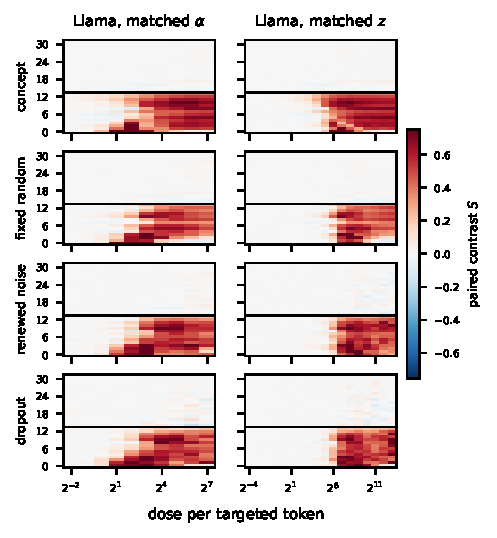
\includegraphics[width=\linewidth]{figures/localization_maps_llama.pdf}
\end{minipage}\hfill
\begin{minipage}[t]{0.48\textwidth}
\centering
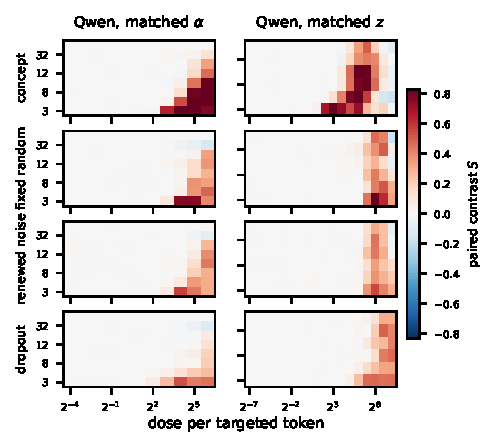
\includegraphics[width=\linewidth]{figures/localization_maps_qwen.pdf}
\end{minipage}
\caption{Paired contrast $S$ on Llama (left) and Qwen (right), one row per
perturbation family and one column per dose rule, with the perturbed block on
the vertical axis and the dose on the horizontal one. Above Llama's rule at
block 14 every cell is neutral at every dose, including standardized doses
that deliver orders of magnitude more raw amplitude than the responsive blocks
require. Qwen decays with depth instead of stopping, and its standardized
column covers the responsive blocks only.}
\label{fig:app-maps}
\end{figure}

\subsection{Where the Scale Is Estimated}
\label{app:loc-scale}

A sentence rendered on its own starts at position 0, where Llama's activation
has norm near 547 against 1.7 to 9.7 everywhere else, and that token is 16\%
of the calibration sample; one concept direction at block 1 projects 582.3
onto it and 0.399 onto every other position. The forced-choice prompt puts the
perturbed tokens at positions 57 to 75, so that token never appears. Concept
vectors are averages of hidden states and inherit the component: their cosine
with the mean position-0 activation runs 0.21 to 0.99, against 0.001 to 0.035
for random directions, which reproduces the measured scale ratio. Qwen does
not do this, and permuting a concept vector's coordinates drops its scale from
1.227 to 0.091 at block 3, onto the fixed-random value of 0.098.
\Cref{tab:app-loc-scales} gives the ratios that dividing by $s(\ell,v)$
removes.

\begin{table}[H]
\centering
\small
\begin{tabular}{llr}
\toprule
Model & Calibration context & concept / fixed random \\
\midrule
Llama & isolated sentence & 22.7--122 \\
Llama & forced-choice prompt & 1.5--3.0 \\
Qwen  & isolated sentence & 5.8--15.8 \\
Qwen  & forced-choice prompt & 3.9--12.6 \\
\bottomrule
\end{tabular}
\caption{Ratio of the median concept scale to the median fixed-random scale,
over the responsive blocks of each model.}
\label{tab:app-loc-scales}
\end{table}

The grid must also reach each family's own threshold, which in $z$ is its
threshold in $\alpha$ divided by its scale: a grid chosen without looking at
the scales reaches one family's transition and not another's, and the untested
families look inert. Each standardized grid here is sized so that its top dose
beats, in every cell, the amplitude that family needs for 75\% correct on the
raw grid.

\subsection{Limits of the Readout}
\label{app:loc-thresholds}

\paragraph{Thresholds.} Only 17 of 508 fitted Llama curves give a threshold
both bracketed and inside the tested range, so no 75\% threshold is quoted for
that model. The curve shape is the cause, not noise: the controls peak before
the top dose and fall 0.16 to 0.21 below a monotone logistic fit, concept
saturates and falls 0.049, and Qwen peaks at $\alpha=16$ at block 3.

\paragraph{Dropout dose.} Its realized rate reaches 0.976 at $\alpha=128$, so
the top doses erase the sentence instead of raising the dose, and the realized
amplitude falls to 99.4 for 128 requested. The three additive families deliver
the request to within $5\times10^{-5}$.

\paragraph{Labels.} Relabeling the two options, with the same sentences, order
and perturbation, moves Llama's $S$ from 0.379 to 0.160 and Qwen's from 0.0593
to 0.0515.

\phantomsection\label{app:loc-contamination}
\paragraph{Leakage.} Leakage from the perturbed sentence to the other
saturates on Llama within two blocks and never decays, with several cells
above 1.0. Attention is causal, so it runs one way and no balancing of trials
repairs it. On Qwen its median is 0.067.

\phantomsection\label{app:loc-scramble}
\paragraph{Scrambled concept.} A concept direction beats its own coordinate
permutation $1.75\times$ at block 3, $+0.445$ against $+0.255$, and
$4.19\times$ at block 6, $+0.300$ against $+0.072$, while the permutation sits
with fixed random at $+0.228$ and $+0.128$. Orientation, not coordinate
statistics, carries the advantage.

\paragraph{Two unexplained results.} Thirteen cells of 2794 sit significantly
below chance, all fixed random, all at Llama's blocks 7 and 12, under both
dose rules. At Qwen's block 32 the families split by sign, concept at $+0.016$
against $-0.013$ to $-0.022$; content does not explain that split, since a
permuted concept vector carries none and still gives the positive sign,
$+0.022$ against $-0.027$. What concept and its permutation share is
heavy-tailed coordinates, kurtosis 6 to 8.5 against 3.
